\section{Analysis of the Problem}  % 一级标题

\begin{figure}[h]  % 图片
\small
\centering  % 居中
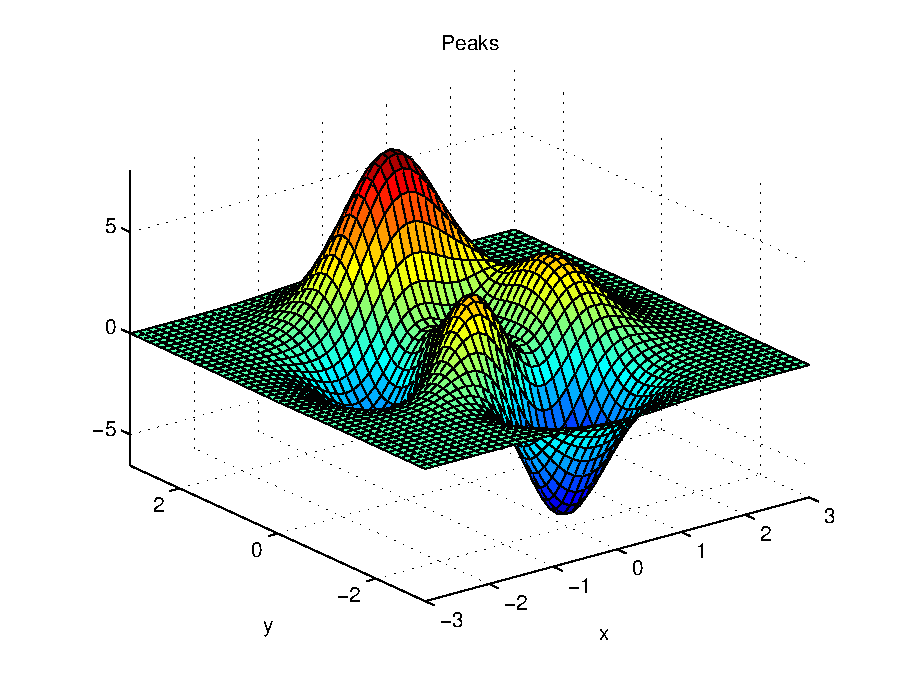
\includegraphics[width=12cm]{example.eps}  % 引入图片源
\caption{example} \label{fig:example}  % 标题与标签
\end{figure}  % 图片结束

This is Figure \eqref{fig:example}.  % 引用图表

This is a cite\cite{vaswani2017attention}.  % 引用文献

\begin{equation}  % 公式,独占一行、居中,自动编号
E = mc^2 \label{aa}  % 标签
\end{equation}  % 公式结束

\begin{equation}  % 公式,独占一行、居中
\nonumber % 不编号
E = mc^2
\end{equation}  % 公式结束

%%%% 并排图
\begin{figure}[h]  % 图片
\centering  % 居中
\begin{minipage}[c]{0.48\textwidth}  % 子页
\centering  % 居中
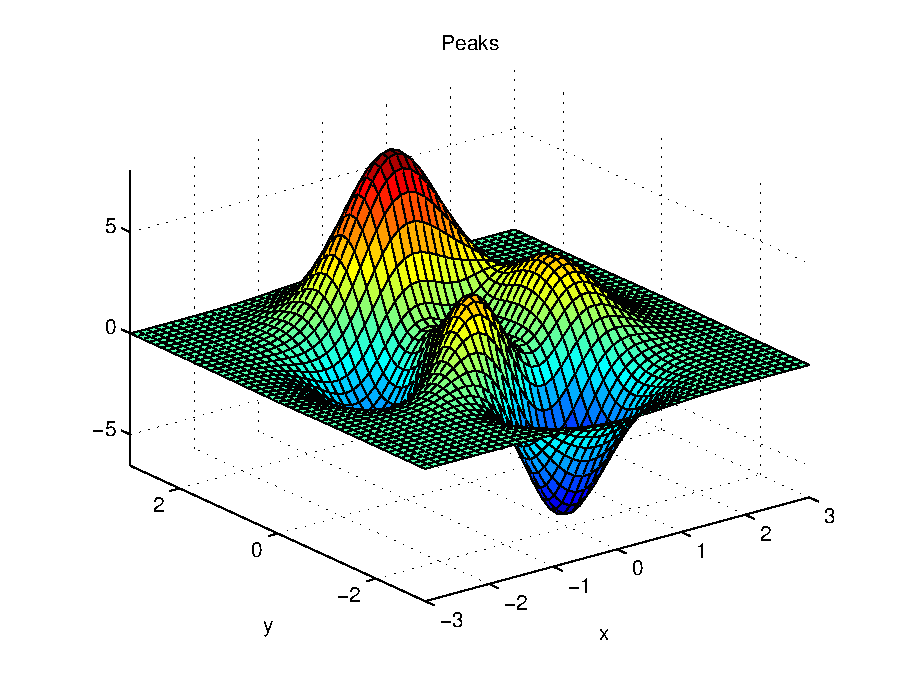
\includegraphics[width=7cm]{example.eps}  % 引入图片源
\caption{example} \label{fig:example}  % 标题与标签
\end{minipage}  % 子页结束
\hspace{0.02\textwidth}
\begin{minipage}[c]{0.48\textwidth}  % 子页
\centering  % 居中
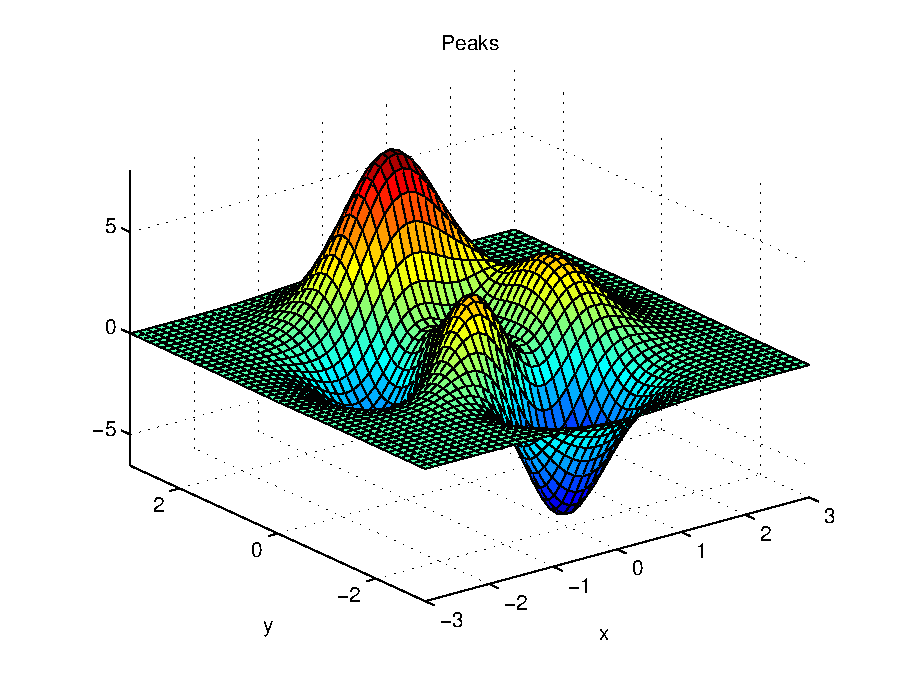
\includegraphics[width=7cm]{example.eps}  % 引入图片源
\caption{example} \label{fig:example}  % 标题与标签
\end{minipage}  % 子页结束
\end{figure}  % 图片结束

%%%% 三线表
\begin{table}[!t]  % 表格
\caption{Caption}  % 标题
\label{tab1}  % 标签
\tabcolsep 42pt % 列间距
\begin{tabular*}{\textwidth}{cccc}  % tabular*环境
\toprule  % 顶线
Title a & Title b & Title c & Title d \\
\midrule  % 中线
Aaa & Bbb & Ccc & Ddd \\
Aaa & Bbb & Ccc & Ddd \\
Aaa & Bbb & Ccc & Ddd \\
\bottomrule  % 底线
\end{tabular*}  % tabular*环境结束
\end{table}  % 表格结束


